\documentclass[11pt,a4paper]{article}
\usepackage[utf8]{inputenc}
\usepackage[T1]{fontenc}
\usepackage{lmodern}
\usepackage[margin=25mm]{geometry}
\usepackage{microtype}
\usepackage{amsmath,amssymb}
\usepackage{booktabs,longtable,tabularx,array}
\usepackage[dvipsnames]{xcolor}
\usepackage{graphicx}
\usepackage{enumitem}
\usepackage{hyperref}
\usepackage{xurl}
\usepackage{fancyhdr}
\setlength{\headheight}{14pt}
\pagestyle{fancy}
\fancyhf{}
\fancyhead[L]{\scriptsize\sffamily\color{CosmicPurple}AGI ALPHA FLYWHEEL}
\fancyhead[R]{\scriptsize\sffamily\color{CosmicPurple}Useful work / measured economics}
\fancyfoot[C]{\small\thepage}
\renewcommand{\headrulewidth}{0.25pt}
\definecolor{CosmicPurple}{HTML}{45236D}
\definecolor{CosmicInk}{HTML}{231534}
\hypersetup{colorlinks=true,linkcolor=CosmicPurple,citecolor=CosmicPurple,urlcolor=CosmicPurple,pdftitle={The Decision That Carries Its Evidence},pdfauthor={AGI ALPHA research lane, MONTREAL.AI; AI-assisted study}}
\setlength{\parskip}{0.35em}
\setlength{\parindent}{0pt}
\setlength{\emergencystretch}{2em}
\setlist{nosep,leftmargin=*}
\newcommand{\Alpha}{AGI ALPHA}
\newcommand{\Successor}{SUCCESSOR $\Omega$}
\newcommand{\TI}{TRANSFORMATIONAL INTELLIGENCE $\infty$}
\newcommand{\Preserved}{\texttt{SCOPED\_COMPONENT\_PRESERVED}}
\newcommand{\Hold}{\texttt{INCOMPLETE\_HOLD}}
\newcommand{\Regression}{\texttt{COMPONENT\_REGRESSION}}
\newcolumntype{Y}{>{\raggedright\arraybackslash}X}
\title{\color{CosmicPurple}\small\sffamily AGI ALPHA FLYWHEEL\\[0.8em]\normalfont\LARGE\textbf{The Decision That Carries Its Evidence}\\[0.6em]\large Useful work, retained capability, and the economic gate in AGI ALPHA}
\author{AGI ALPHA research lane, MONTREAL.AI\\\small AI-assisted research, engineering and publication study}
\date{26 October 2026}
\begin{document}
\maketitle
\begin{abstract}
A maintainer needs to know whether a dependency proposal preserves the application properties that matter. We construct and execute a bounded answer for the actual \Alpha{} request boundary and mission-input models, then retain the capability that produces the answer with its source, observations, verification and next action. The first useful result assesses the native component profile against a proposed refresh through the original FastAPI import bridge. A source-grounded contract covers 21 request-boundary and 40 model cases, including the actual 15-second body timeout. After discovery, criticism and correction, we freeze 83 source files and compare the study's researcher-assisted incumbent (A), an automated retained producer (B), and a strong conventional reusable \texttt{unittest} builder (C). Six previously uninspected historical dependency transitions in two package clusters yield eighteen evaluations. All three methods deliver six accepted scoped-preservation packets; B and C remove the six explicit researcher finalizations required by A. Median request-to-package spans are 36.220, 16.554 and 16.628 seconds respectively, but A includes researcher response and scheduling waits and is not a human-without-AI benchmark. A's mechanical median is 16.310 seconds. The result supports useful automatic packet completion, not an exclusive method advantage or a priced labor saving. Complete monetary construction, delivery and maintenance costs remain unidentified; actual customer collections are zero. The canonical economic gate remains HOLD. The contribution is an executable consumer decision, a retained evidence-bound delivery asset, and a reproducible separation of engineering reuse from investment repayment.
\end{abstract}

\section{The useful outcome comes first}

The offering investigated here is one \emph{component-compatibility decision packet} for an exact consumer revision and a substantive dependency proposal. A maintainer receives the question, the requirements being checked, original source identities, exact before/after component environments, executable observations, an independent finite-contract decision, a reviewable component-lock patch and the next justified action. This is work that a competent engineer can perform with ordinary tests, source inspection, dependency metadata and existing caches. The service question is whether automation can deliver that accepted work repeatedly and whether retaining the capability is worth its complete cost.

For the actual \Alpha{} source, the first useful result is concrete: the proposed development refresh preserves the declared \texttt{RequestBoundary}, \texttt{Mission}, \texttt{Review} and \texttt{Control} properties in the tested environments. The appropriate action is to accept this component evidence for further application qualification while keeping the current native lock. It is not an authorization to deploy the proposed tuple. The original source and native tests make request framing, byte bounds, origin checks, timeouts, strict mission inputs and response headers consequential properties, rather than arbitrary benchmark tasks.\cite{consumer,contract,firstdelivery}

\begin{table}[htbp]
\centering\small
\begin{tabularx}{\textwidth}{@{}p{0.21\textwidth}YY@{}}
\toprule
Customer question & Supplied evidence and action & Remaining responsibility \\
\midrule
Does this exact proposal preserve the declared component properties? & Source-bound before/after observations, all requirement results, a scoped verdict and replayable artifacts. & Decide whether the refresh is needed and whether this scope addresses the actual maintenance question. \\
Can the proposal move to the next qualification stage? & If complete and conforming, advance the component evidence; if a required behavior fails, hold the proposed tuple with its reproduction. & Qualify the complete dependency lock, supported platforms, authentication, persistence and real mission execution. \\
Can the release be adopted? & The packet explicitly preserves owner and exact-source release gates. & Existing owners and integrators decide release and operator adoption. \\
\bottomrule
\end{tabularx}
\caption{The accepted product is a bounded decision with evidence. Customer and release acceptance are separate events.}
\label{tab:offering}
\end{table}

The source requirement is an observed internal project need. Published dependency changes provide real triggers. The selected historical transitions are representative maintenance assessments, not six observed Alpha adoptions, purchase orders or instances of paid demand. The first native-profile refresh is a development example, and the historical confirmation set is a different evidence class. An unchanged valid request is normally a no-op; changing an assertion, rendering the same result twice or repeating a measurement does not create another mission.\cite{selection,protocol}

The addressable work therefore starts narrowly: maintainers of compatible Python components who need this exact requirement-and-evidence package. It does not extend experimentally to all software maintenance, migrations or enterprise operations. No numerical market size, obtainable demand, monthly capacity, price or reinvestment share is inferred from the existence of this work. Broader upgrade services provide context for the category, while their larger scope prevents direct price substitution (Section~\ref{sec:human}).

\subsection{Precise contribution}

This study contributes (i) an executed, source-grounded decision for actual consumer components, including a finite independently specified behavioral contract; (ii) a retained producer that constructs the decision together with its evidence and integrates through an existing local \Successor{} Workbench seam; and (iii) a frozen comparison against both a complete researcher-assisted incumbent and a strong conventional reusable builder, coupled to one finite cost and financing account. It also preserves the failures that motivated and corrected the asset. The result does not establish general intelligence, autonomous invention, economic admission, better construction of a next capability or sustained acceleration.

\section{From a useful first delivery to a justified structural change}
\label{sec:first}

\subsection{The first native-profile assessment}

The experiment uses the original consumer definitions at Alpha revision \path{eb07086ac42799ff45f7b1c946a2f7c514bd3bbc}. A later source handoff rechecked identical consumer, test and native-lock Git blobs at \path{92064005b55d4fec0effbb2acacc8403bb551f3e}; this equality supplies provenance, not a new experimental mission or release qualification.\cite{consumer,companion}

The native component environment contains FastAPI 0.141.1, Starlette 1.7.0, Pydantic 2.13.5 and pydantic-core 2.46.5. The development proposal changes the last three to Starlette 1.10.0, Pydantic 2.14.1 and pydantic-core 2.50.1. The unchanged support closure is anyio 4.15.1, annotated-types 0.8.0, typing-extensions 4.16.0, typing-inspection 0.4.4, idna 3.20 and annotated-doc 0.0.5. Each distribution is pinned to an official published wheel identity. Both exact environments satisfy the 61 declared cases.\cite{firstdelivery,selection}

The request-boundary cases cover valid fragmented bytes, the exact 524,288-byte limit, malformed or conflicting framing, excess declared or actual size, origin handling, disconnects, body replay and security headers. The downstream recorder deliberately emits a weak cache-control value so the original boundary must replace it. The actual configured 15-second timeout executes without shortening the constant or substituting a fake clock. Model cases cover strict scalar types, forbidden extra fields, bounds, discriminated work variants, duplicate identifiers, forecast relations and finite values, complete accepted serialization, and inert Review/Control input validation. Expected rejections are correct guard behavior, not newly discovered production defects.\cite{contract}

No full application is created. In particular, the experiment does not initialize a Journal, create credentials, exercise the complete authentication or trusted-host stack, persist a real mission, or perform an approval/control action. The original native test file contains some of these broader operations; our component probes do not claim to run that file unmodified. Its requirements inform a narrower explicitly enumerated contract.\cite{consumer,contract,criticism}

\subsection{What was missing from the preceding source-only lane}

The preceding \emph{Next Upgrade} lane produced source-level compatibility reports. Independent criticism identified a consequential obstruction to the broader consumer decision. Its pipeline generated declaration reports only for changed modules, while its consumer mapper needed signatures for actual consumer calls, including unchanged modules. In a preserved FastAPI example, 38 of 57 dependency-import references resolved to declarations in captured but unchanged modules and therefore lacked a supplied signature; the other 19 stopped at uncaptured Starlette exports. Those counts identify a construction omission, not proof that all calls would pass a full binding checker if signatures were supplied.\cite{criticism,nextupgrade}

That same packet recorded 10,172 unresolved calls, zero established preserved bindings and zero established consumer losses. Its readiness status reflected its narrower source-report contract. It explicitly did not approve production. We therefore preserve the earlier result and its correct scope, rather than relabeling it as a failed behavioral assessment. A report about changed declarations does not by itself answer whether the application's required behavior is preserved.\cite{criticism}

Three candidate changes were screened. Consumer-first source/export closure could improve static completeness but could not establish runtime behavior by itself. A requirement-linked executable component decision could answer a concrete maintenance question within the authorized environment. A general dynamic dispatch analyzer was rejected as too broad for the bounded contribution. Earlier polling/cache opportunities were also rejected as insufficiently material to support a new economic claim. Discovery and rejected approaches remain chargeable records; the primary was not selected from favorable confirmation outcomes.\cite{discovery}

\subsection{The retained structural change}

The retained representation combines the job's source identities, exact environment pair, finite contract, observations, verifier results and decision. Packaging is part of the deliverable, rather than a later unsupported interpretation of an upstream report. A preserved verdict requires complete bound evidence; an attributable target mismatch leads to a negative assessment; incomplete evidence cannot become approval. The actual implementation includes a paired execution controller, process receipts, an independent verifier, a decision/evidence assembler and a registered local Workbench adapter.\cite{companion}

The asset was constructed with model-assisted research and engineering. It was not autonomously invented by a deployed enterprise. The conventional builder independently implements an ordinary \texttt{unittest} recorder and package assembler using the same sources, requirements, environments, verifier, permissions and reusable-asset rights. Its stronger receipt checker was subsequently adopted inside the retained producer. That adoption is evidence of useful criticism and conventional component reuse, not evidence that the custom method invented a superior validator.\cite{controls}

\section{A connected productive cycle with consequential criticism}

\TI{} is used here through concrete work products. \emph{Identify} selects the consumer's dependency decision; \emph{Out-Learn} examines source, native tests and the limitations of prior outputs; \emph{Out-Think} distinguishes a declaration report from behavioral evidence; \emph{Out-Design} binds the decision to the actual executable contract; \emph{Out-Strategise} fixes the comparator, untouched-input rule and cost gate; \emph{Out-Execute} produces and independently checks the packet; \emph{Out-Evolve} incorporates substantiated corrections and tests the retained asset on the frozen new work. Each stage has an artifact or decision consequence. The vocabulary does not turn this engineering sequence into a proof of intelligence or acceleration.\cite{discovery,criticism,protocol}

Critic agreement alone was insufficient. The critic supplied a source location, a consequential discrepancy and its relevance to the intended outcome; a separate verifier adjudicated it. The first baseline used an eight-package direct-Starlette import projection. Although its observations passed the initial cases, the critic showed that it bypassed the original FastAPI import bridge. The correction restored FastAPI and annotated-doc in the ten-package closure before primary freeze. The provisional result remains preserved and is not counted as native-import qualification.\cite{criticism,firstdelivery}

A second criticism concerned contemporaneous provenance. The earliest execution receipt recorded time, command and output but did not bind every worker, interpreter and lock byte before execution. Current file hashes cannot retroactively establish those earlier identities. The corrected meter records pre/post input identities and output hashes; the package checks the required inventory rather than accepting a generic successful exit. The original weaker record remains intact.\cite{criticism}

\begin{table}[htbp]
\centering\small
\begin{tabularx}{\textwidth}{@{}p{0.23\textwidth}YY@{}}
\toprule
Confirmed problem & Consequence demonstrated & Correction before freeze \\
\midrule
Incomplete provenance accepted by initial B & Five malformed provenance variants still produced accepted preservation packets. & Adopt C's strict receipt checker and enforce exact job, worker, source and manifest identities. \\
Verifier exit 2 treated as missing custody & A complete behavioral mismatch could not reach the promised regression decision. & Use typed phase-specific exit sets: worker 0/1, verifier 0/2; retain launch and timeout refusals. \\
Import projection omitted original FastAPI bridge & Component observations could be mislabeled as the native import closure. & Restore original imports and ten exact packages; rerun both development environments. \\
\bottomrule
\end{tabularx}
\caption{Criticism changes implementation or claim scope only when supported by source and executable evidence.}
\label{tab:criticism}
\end{table}

The initial retained-custody control set passed 3 of 9 controls. After correction, 14 of 14 focused controls passed. The additional controls include an unstarted command, wrong arm, missing required manifest entry and a boolean masquerading as an integer exit code. A labeled semantic-observation fault passed through the real independent verifier and produced \Regression{} with complete custody. That observation was manufactured for a control; no new consumer dependency defect or repair is attributed to it. Five variants of the provenance mechanism are not five independent consumer defect families.\cite{controls}

These corrections provide a small structural ablation: removing required receipt checks changes admission of malformed evidence, and repairing the phase-specific exit predicate changes whether a complete negative assessment is deliverable. They do not prove an economic advantage. The new baseline and the strong conventional asset are both retained, and their construction, failed attempts, integration and scrutiny remain in the account.

\section{Frozen comparison and acceptance}
\label{sec:design}

\subsection{Missions and freshness}

Release metadata were fixed at 14:33:37 UTC on 26 October 2026. For each of Starlette major 1 and Pydantic major 2, the curator chose the latest four eligible stable non-yanked versions with compatible Python 3.12 wheel metadata after excluding known body/runtime exposures and development versions. Three adjacent \emph{eligible} transitions per package define six missions. Intervening excluded releases are disclosed; for example, native/development Starlette 1.7.0 is not a held-out body between 1.6.0 and 1.8.0. Pydantic's exact pydantic-core dependency is an explicit coupled change, not a hidden independent intervention.\cite{selection}

\begin{table}[htbp]
\centering\small
\begin{tabular}{@{}llll@{}}
\toprule
Mission & Changed package & Before & After \\
\midrule
Starlette 1 & Starlette & 1.5.1 & 1.6.0 \\
Starlette 2 & Starlette & 1.6.0 & 1.8.0 \\
Starlette 3 & Starlette & 1.8.0 & 1.9.0 \\
Pydantic 1 & Pydantic / core & 2.13.2 / 2.46.2 & 2.13.3 / 2.46.3 \\
Pydantic 2 & Pydantic / core & 2.13.3 / 2.46.3 & 2.13.4 / 2.46.4 \\
Pydantic 3 & Pydantic / core & 2.13.4 / 2.46.4 & 2.14.0 / 2.50.0 \\
\bottomrule
\end{tabular}
\caption{Six substantive historical dependency transitions. The consumer, requirements and other component versions remain fixed as declared.}
\label{tab:missions}
\end{table}

The primary protocol and 83-file source epoch were frozen at 15:17:08 UTC before any selected package body or runtime outcome was acquired. A command-expansion and measurement driver was separately sealed before the first primary behavior. No failed acquisition or evaluation could be replaced based on its outcome. The public freeze record and local manifests bind this sequence.\cite{freeze,protocol}

Held out means no package-body or outcome inspection by this study's builders before freeze. The releases were public historical artifacts and may have appeared in model training. The consumer source, common support packages and contract were deliberately exposed. This is not a prospective field trial, a secret benchmark or six independent defect families.

\subsection{Three complete alternatives}

\textbf{A: researcher-assisted incumbent.} The actual first-completion workflow created during this study provides the incumbent. It retains the original probe, exact environments, common verifier, reusable templates and saved assembly pattern. A one-time charged parameterization avoids forced retyping across six missions. The root researcher inspects the common verifier outcomes and supplies the disposition explicitly; the template rejects an unsupported disposition. A is not a recruited human performing the task without AI, nor a preexisting commercial service whose development was free.\cite{incumbent}

\textbf{B: retained producer.} B uses the same original recorder as A and automatically constructs the evidence-bound decision and English/French HTML package. It uses the common paired controller, independent verifier and adopted conventional receipt checker, then returns the complete artifacts through the registered local Workbench adapter.\cite{companion}

\textbf{C: strong conventional builder.} C independently implements the component exercise with standard-library \texttt{unittest} and a complete bilingual Markdown package. It can use the same sources, tools, environments, requirements, caches, concurrency and reusable-asset construction rights. Its recorder preserves detailed raw ASGI traces in addition to the required observations. It shares the common verifier and infrastructure, so independence is not claimed for every downstream decision component.\cite{conventional}

All builders may reuse a valid prior baseline observation when the consumer, contract, environment, worker and verifier identities and complete custody chain match. These implementations elected to execute both sides freshly in parallel; reuse was not forbidden to weaken C. Identical whole jobs remain no-ops. Each new builder's construction is charged, including C's validator used by B and A.\cite{protocol,incumbent}

\subsection{Quality and resource envelope}

The common contract contains 61 requirements, not 61 customer jobs. It verifies exact case inventory, observed values, full accepted model output, type distinctions, original constants, source projection, environment versions and required response headers. A complete preserved baseline and complete target mismatch can yield an accepted negative assessment. Missing cases, stale identities, launch errors, timeouts or unresolved required fields yield \Hold{}. A successful process exit alone is insufficient.\cite{contract}

Execution uses Python 3.12 on Linux x86\_64, two concurrent before/after workers, a 45-second worker budget and bounded enclosing delivery. The 15-second body timeout supplies a real floor to the observed pair duration. The six missions run in a balanced arm order, one timing execution per arm and mission. The study does not compute a significance test or a generalized reliability rate from this small, clustered historical sample.\cite{protocol}

The primary timing unit is request-to-complete-package span. For A it includes the researcher's response and scheduling; the paired execution plus finalization commands supply a distinct mechanical duration. B/C enclosing receipts and their workers are nested measurements, not additive bills. Shared environment acquisition is charged once. Human attention, remote inference billing and complete customer turnaround are not inferred from these clocks.\cite{economics}

\section{Results: useful automation, ordinary methods remain strong}
\label{sec:results}

All eighteen evaluations completed with \Preserved{}. Each arm delivered six accepted scoped packets, with 61 conforming cases before and 61 after for each mission. No primary target regression, missing-case hold or acquisition failure occurred. Internal acceptance is tied to the finite contract; no maintainer/customer acceptance or production adoption was observed. The complete result matrix and every packet remain available.\cite{results,productreview}

\begin{table}[htbp]
\centering\small
\begin{tabularx}{\textwidth}{@{}Yrrr@{}}
\toprule
Measure & A: manual & B: retained & C: conventional \\
\midrule
Accepted scoped packets / missions & 6/6 & 6/6 & 6/6 \\
Explicit researcher finalizations & 6 & 0 & 0 \\
Median service span (s) & 36.220 & 16.554 & 16.628 \\
Service span range (s) & 25.809--50.462 & 16.439--16.669 & 16.530--16.758 \\
Median mechanical duration (s) & 16.310 & 16.506 & 16.576 \\
Median measured local CPU (s) & 1.786 & 2.043 & 2.085 \\
Total measured local CPU (s) & 10.770 & 12.094 & 12.643 \\
Complete monetary cost & Unknown & Unknown & Unknown \\
Actual customer collections & 0 & 0 & 0 \\
\bottomrule
\end{tabularx}
\caption{Descriptive single runs on a shared host. A's service span includes response/scheduling wait; its mechanical duration is lower than B's median. CPU includes the terminal's enclosing child and controller quantities once. Neither service differences nor CPU seconds identify wages, inference charges or savings.}
\label{tab:results}
\end{table}

\IfFileExists{figures/outcome-matrix.pdf}{\begin{figure}[htbp]\centering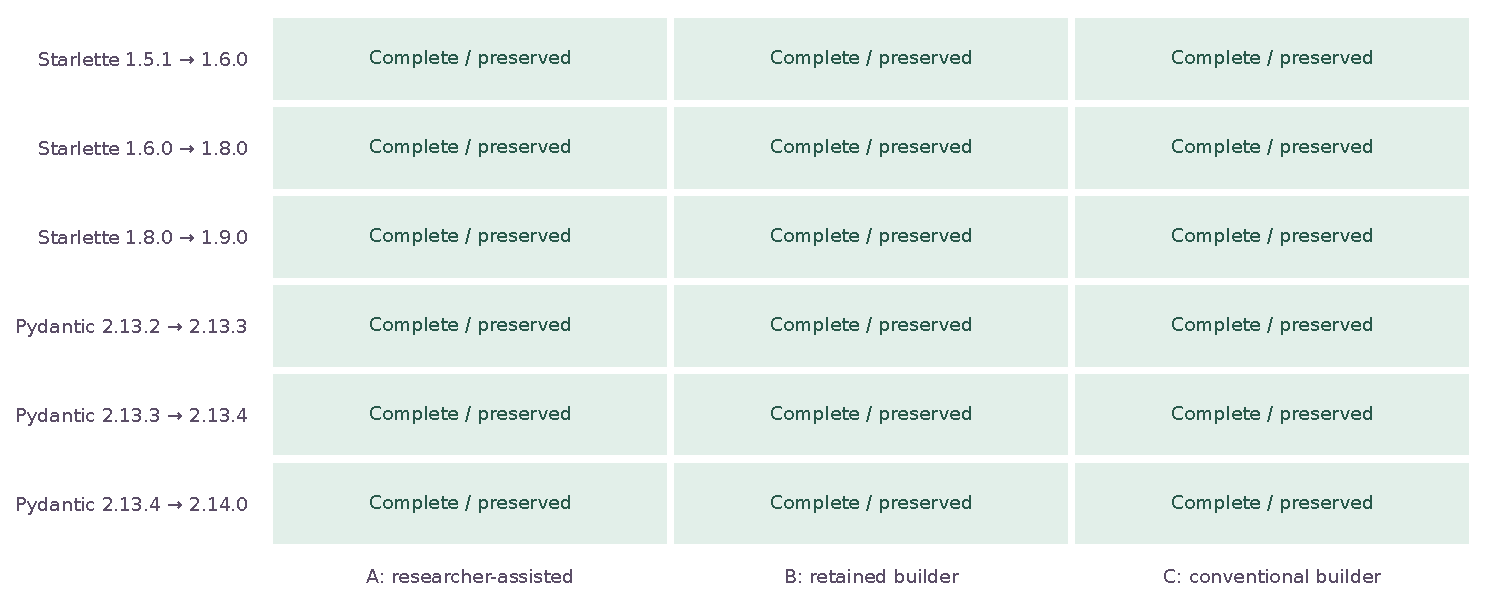
\includegraphics[width=\textwidth]{figures/outcome-matrix.pdf}\caption{The six mission outcomes under all three methods. Assertions and method evaluations do not increase the distinct workload count.}\end{figure}}{}
\IfFileExists{figures/resource-comparison.pdf}{\begin{figure}[htbp]\centering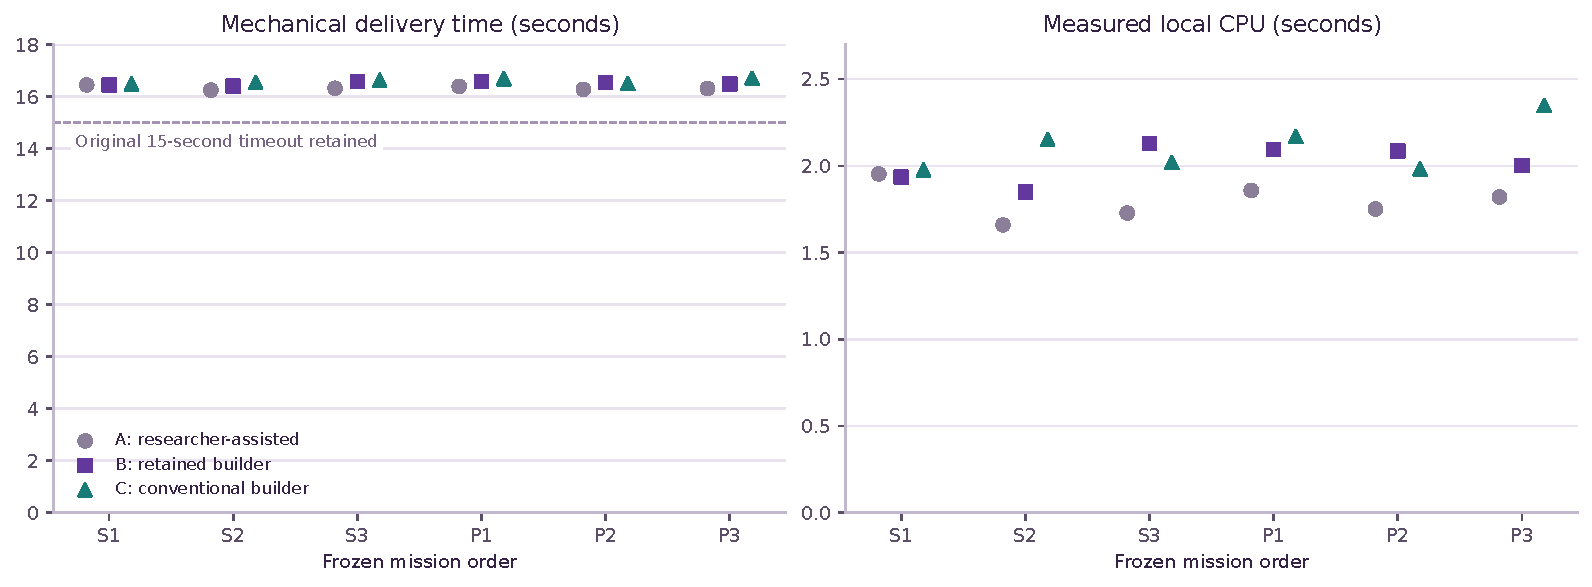
\includegraphics[width=\textwidth]{figures/resource-comparison.pdf}\caption{Observed mechanical delivery time and local CPU. The original 15-second timeout is retained. Researcher-containing service spans are reported separately in Table~\ref{tab:results}; these panels do not measure priced attention savings.}\end{figure}}{}

The operative improvement is removal of an explicit finalization intervention in the study incumbent while delivering the same accepted scope. Both B and C achieve it. A and B retain the same recorder and oracle, but templates, packaging and orchestration differ, and the researcher is not blind to earlier arms. Thus the comparison supports the recorded intervention change; it does not isolate a universal turnaround effect or identify human minutes saved. All arms eventually produce the same number of accepted outputs.\cite{protocol,results}

C's performance and acceptance show that ordinary reusable test tooling is a strong way to deliver the product. The small B/C timing differences are single-run observations on a shared host, with different trace serialization and packaging. We do not call them an algorithmic breakthrough. B also consumes more measured local CPU in aggregate than A. Charging only the smaller automatic service span and ignoring construction, validation or the manual scheduling interval would produce a misleading economic conclusion.

Eight exact confirmation profiles were prepared with no failed attempts, using 16 recorded requests and 11,124,909 response bytes. The acquisition driver records 30.922 seconds of wall time, 29.664 seconds of inclusive child CPU and 0.019 seconds of its own CPU. Inner preparation records are diagnostic and are not charged a second time. These are physical resource observations, not a full monetary bill.\cite{economics}

A reporting reviewer inspected all terminal-marked English/French packets, finding no consequential discrepancy between next action and scoped decision, no terminal-to-decision hash mismatch and no broken local HTML download/language link. The reviewer authored C and A's parameterization and discloses that role. Separate source/custody and economic scrutiny provide different checks. The compact B HTML's generic component naming and French resource wording are presentation qualifications carried into the publication overlay; original frozen outputs are preserved.\cite{productreview}

The separate final custody review passed all eighteen packets, including enclosing and inner receipt bindings, manifests, case inventories, patches and embedded native artifacts, with all 83 frozen files unchanged. All twelve native B/C runs retain HOLD, empty authority and disconnected settlement; their inspection status remains \texttt{UNAUTHENTICATED\_HISTORICAL\_IMPORT} with empty active proof and authority. Artifact consistency does not convert those records into an authenticated operator history. The independent economic aggregation audit also passed.\cite{custody,economicaudit}

\section{The complete operating model and the economic gate}
\label{sec:economics}

Primary outcome tables use immutable accounting snapshot 01. Lifecycle snapshot 02 adds completed publication and scrutiny resources through 26 October 2026, 15:42:59 UTC, while preserving the same primary values. Later delivery verification and publication work are recorded in an additive supplement to the same study-investment account. Unmeasured and still-open lifecycle items remain unknown; the snapshot cutoff is not a claim that later reporting, storage or maintenance is free.\cite{economicupdate}

\subsection{What is automated and what is not}

For registered permitted jobs, paired component execution, observation verification, required receipt checks and B/C packet assembly are automated. Environment construction and exact package acquisition are scripted and measured. Source selection, scope design, oracle creation, unsuccessful construction, review and publication were model-assisted research work; their inference bills and active attention are unknown. Customer selection of a needed proposal, input preparation beyond this prepared study, acceptance, and full application qualification remain separate work. No permanent staffed service is assumed to make the result positive, and no residual activity is silently assigned zero cost.\cite{economics,companion}

The finite investment account covers this actual component-assessment asset: discovery and rejected candidates; the initial manual delivery; both reusable builders; common execution, measurement and verification; the provisional import profile and its correction; the failed initial B custody implementation; adoption of C's checker; environment preparation; scrutiny; integration; delivery; failed attempts; publication; and future attributable upkeep. The accounting distinguishes nested receipts, immutable evidence copies and actual new execution. Assistant timestamps provide documentary provenance, not additional CPU bills or human wages.\cite{economics}

The numerical primary tables cite immutable economic snapshot 01. Publication and later reproduction have additional recorded costs; subsequent append-only accounting snapshots can extend that inventory without altering the primary outcomes. A complete monetary total is not inferred from the snapshot's partial physical subtotals.\cite{economicaudit}

\begin{table}[htbp]
\centering\small
\begin{tabularx}{\textwidth}{@{}p{0.24\textwidth}YY@{}}
\toprule
Cost level & Observed basis & Remaining uncertainty \\
\midrule
Marginal execution & Complete local delivery spans and CPU, worker/verifier receipts, accepted outcomes and failures. & Monetary compute/storage rate, any attributable billing outside the captured process envelope, customer input/review effort. \\
Recurring delivery & Reusable code and exact environments; scripted acquisition and explicit maintenance/requalification triggers. & Justified utilization, recurrence, shared upkeep, exceptions and service obligations. \\
Fully loaded asset & Construction and correction records, both builders, common scrutiny, failed B attempts, integration and publication. & Complete model/token invoices, active research attention, legacy/shared allocation and future maintenance. \\
\bottomrule
\end{tabularx}
\caption{Unknown is distinct from zero. The companion reports known physical subtotals and missing quantities, rather than a fabricated complete price.}
\end{table}

The preserved canonical accounting closure computes cost and financing states without changing its arithmetic. Its upstream modules are source candidates from held integration work, not newly claimed released services. The adapter retains all eight operating stages and separates starting capital, collections, delivery, investment, obligations, reserves and available surplus. In the actual account, customer collections and new paid commitments are zero; starting funded capital, complete costs, obligations, reserves and unencumbered funds remain unidentified. The economic admission is HOLD, and monetary repayment and financeable expansion are not established.\cite{canonical,economics}

\subsection{One investment, a finite payback question}

For the same accepted deliverable, let $I$ be complete incremental investment in the retained asset, $C_{A,j}$ and $C_{B,j}$ the complete attributable delivery costs, and $m_j$ incremental maintenance over a justified finite horizon $N$. The relevant net benefit is
\begin{equation}
V(N)=\sum_{j=1}^{N}\bigl(C_{A,j}-C_{B,j}-m_j\bigr)-I.
\label{eq:payback}
\end{equation}
Equivalent accepted outcomes and the costs of failed attempts are prerequisites to interpreting $V$. In a constant conditional case with per-mission saving $s$ and maintenance $m$, a positive $s-m$ gives
\begin{equation}
N_{\mathrm{break\ even}}=\left\lceil\frac{I}{s-m}\right\rceil.
\end{equation}
If $s-m\leq0$, a positive investment has no finite payoff under that assumption. Here $I$, $s$, $m$ and a justified demand horizon are unknown, so no numeric crossing is supported. Small local CPU differences cannot identify these terms. A favorable assumed attention saving is not inserted to rescue the result.\cite{economics}

\begin{table}[htbp]
\centering\small
\begin{tabularx}{\textwidth}{@{}p{0.23\textwidth}YY@{}}
\toprule
Sensitivity & Directional implication & What this study identifies \\
\midrule
Low utilization & Fixed construction and recurring shared cost are allocated over fewer accepted deliveries. & No utilization or amortization horizon is assumed. \\
Maintenance & Requalification and repair increase $I$ or $m_j$; stale assets cannot retain admission by assertion. & Triggers are explicit; future frequency and complete cost are unknown. \\
Failure and correction & All attempts remain in the cost numerator; incomplete output earns no accepted-delivery credit. & Development failures are retained; six primary transitions do not estimate a deployment failure rate. \\
Demand & An unused capability cannot generate customer collections. & Zero paid orders and receipts observed; recurring release metadata is not paid recurrence. \\
Attention & A real measured reduction might be economically material. & No active-time measurement or same-scope willingness to pay; contribution to a favorable savings model is not invented. \\
\bottomrule
\end{tabularx}
\caption{Sensitivity without arbitrary prices, invented recurrence or unmeasured attention savings.}
\end{table}

A positive value calculation would still not be spendable cash. At time $t$, the finite cash account is
\begin{align}
B_t &= B_{t-1}+R_t+K_t-D_t-J_t,\\
A_t &= B_t-O_t-Q_t,
\end{align}
where $R_t$ is actually collected revenue, $K_t$ authorized external capital, $D_t$ paid delivery cost, $J_t$ paid investment, $O_t$ unpaid obligations and $Q_t$ required reserves. Customer savings, token principal, appreciation and accounting allocations are not $R_t$. No transaction, token operation or newly paid commitment occurs here. Unknown balances cannot authorize expansion.\cite{economics,ecosystem}

\section{Comparison with competent human work}
\label{sec:human}

A human without AI could use the existing tests, Python tools, Git, lockfiles and dependency metadata to produce an equivalent component packet. Dependabot supplies version-update proposals; Griffe supplies declaration-change evidence; ordinary reusable test suites can execute the application's requirements. These tools remain practical alternatives. Their availability does not make implementation, interpretation, infrastructure or accepted responsibility free. Conversely, our narrow automatic check does not replace all responsibilities of a software quality professional.\cite{dependabot,griffe,human}

No matched human task duration was measured. A is an observed researcher-assisted workflow constructed in this study, with charged new helpers and an explicit decision step. Treating A's 36.220-second median service span as a no-AI labor benchmark would confuse waiting, scheduling, automation and active work. A recruited panel is unnecessary for an explicitly modeled threshold, but a precise savings ratio requires evidence that we do not have.

The U.S. Bureau of Labor Statistics reports a May 2025 median hourly wage of USD~50.14 for software quality assurance analysts and testers. The preserved same-day Canadian source record reports CAD~46.26 for the broader NOC~21222 software-QA category in Montr\'eal, with a 2024 reference period. These are wages, not consulting prices or fully loaded employer costs; the currencies and occupational definitions remain separate.\cite{bls,jobbank,human}

For equivalent accepted human work lasting $t$ minutes at wage $w$, the wage-only modeled cost is $H=wt/60$. If complete automated provider cost is $C$, the crossing occurs at
\begin{equation}
t^*=60C/w.
\end{equation}
The coefficients are 1.19665 minutes per USD at the U.S. median and 1.29702 minutes per CAD at the Montr\'eal median. These are algebraic coefficients, not measured task durations. Because $C$ remains unknown, the actual crossing remains unknown. Customer savings require a different comparison: actual price plus customer effort against an equivalent alternative, preserving differences in coverage and responsibility.\cite{human,economics}

An adjacent vendor advertises a \$1,500 Django upgrade assessment covering code, dependencies, test coverage and deployment, with a written plan and upgrade quotation. This is a broader advertised service, not an observed transaction, a clearly specified currency, a no-AI benchmark, or a price for our component packet. We do not subtract our unpriced CPU run from that amount. The category is commercially recognizable, but a same-scope buyer and price are unobserved.\cite{netlandish}

\section{Reuse, succession and the next justified allocation}

A connected productive cycle has been executed: a useful component decision was identified and delivered; its limits and resources were recorded; the missing evidence-to-action construction was diagnosed; a retained producer was built and corrected; untouched historical work was evaluated; and successful scoped packet production was reused. Admission here means eligibility for this local research workflow under the frozen contract. Native operator, release and economic gates retain their separate HOLD or approval requirements.\cite{results,ecosystem}

Four different claims must remain separate. Better completion of the stated task is supported by the new executable consumer packet, with the earlier source-only scope preserved. Useful capability reuse is supported by repeated complete delivery on six substantively changed tuples and removal of the incumbent's explicit finalization. Better construction of another capability has not been tested under comparable new construction problems. Sustained acceleration across economically funded cycles has not been established. None follows automatically from a successful cache, repair, repeated schedule or ledger replay.

The next justified work is a real pending matching maintenance decision. Before execution, a maintainer should identify the needed action, exact consumer revision, permitted inputs and accepted scope. Record active input preparation, review, exceptions, complete resource and billing evidence where available, and whether the packet was actually used. A competent ordinary workflow retains its tools and caches. If a later authorized buyer provides a scope-matched quote or allocation, preserve price, acceptance, payment and funding authority separately. This study creates no outreach, payment or new commitment.\cite{human}

The asset should be requalified when its source, requirements, import bridge, dependency bytes, runtime platform, rights or receipt assumptions change. Unsupported scope or unverifiable evidence produces an explicit hold, with the preserved complete manual workflow as fallback. Retire active use when the need disappears or observed complete maintenance cost is not justified by useful demand; preserve historical failures and receipts. Engineering usefulness deserves reuse only within those limits. Investment repayment requires the additional evidence set out in Equation~\ref{eq:payback}.

\section*{R\'esum\'e en fran\c{c}ais}

Le r\'esultat utile est un dossier de compatibilit\'e des composants pour une proposition pr\'ecise de mise \`a jour. Il r\'eunit le code source d'origine, les d\'ependances exactes, les exigences, les observations avant et apr\`es, une v\'erification ind\'ependante et la prochaine action justifi\'ee. Le premier exemple AGI ALPHA ex\'ecute les propri\'et\'es d\'eclar\'ees de \texttt{RequestBoundary}, \texttt{Mission}, \texttt{Review} et \texttt{Control}, avec le chemin d'importation FastAPI d'origine et le d\'elai r\'eel de quinze secondes.

Les trois m\'ethodes produisent chacune six dossiers accept\'es dans ce p\'erim\`etre. Les deux solutions r\'eutilisables suppriment les six finalisations explicites du chercheur requises par le flux initial. La solution conventionnelle obtient les m\^emes r\'esultats; aucune sup\'eriorit\'e algorithmique exclusive n'est d\'emontr\'ee. Les dur\'ees du flux manuel comprennent les attentes de r\'eponse et d'ordonnancement et ne mesurent pas le travail d'un professionnel sans IA.

Une d\'ecision positive permet d'accepter les preuves limit\'ees aux composants et de poursuivre la qualification compl\`ete de l'application, en conservant le verrou natif actuel. Elle n'autorise ni publication ni exploitation. Les ressources mesur\'ees sont conserv\'ees; les co\^uts mon\'etaires complets, le prix, le temps d'attention et la demande restent inconnus. Les encaissements clients sont nuls. La r\'eutilisation d'ing\'enierie est \`a distinguer du remboursement de l'investissement, d'un surplus disponible et d'une acc\'el\'eration durable.

\appendix
\section{Exact methods and source-execution boundary}

The probe extracts the declared API definitions and constants from the pinned AST and uses the original model definitions. The projection inventory records their hashes and the original import-header AST identity. Imports retain FastAPI's \texttt{Request} and \texttt{JSONResponse} bridge and Starlette's ASGI types. The recorder does not rewrite the request-boundary algorithm in its own implementation. Trusted published pinned dependency packages execute in isolated component environments; no arbitrary user bundle, operator home or authenticated service is executed.\cite{contract,companion}

The ASGI recorder scripts local receive events and a harmless in-process downstream response. It distinguishes exact byte counts and hashes, downstream entry count, response messages and required headers. A disconnect can correctly emit no response. The original timeout, body limit and strict-model settings remain bound to the source. For model validation, \texttt{model\_validate} and \texttt{model\_validate\_json} are distinct cases. NaN and positive/negative infinity are materialized as actual floating values only for declared Python-input cases; tags or strings are not substituted. The verifier compares complete outputs with JSON scalar types preserved, so a boolean cannot silently stand in for an integer.\cite{contract}

Before/after workers run concurrently under the same envelope. Each process receipt binds worker, verifier, contract, projection, consumer, lock, preparation record and interpreter as required; output identities are checked after completion. The package imposes the inventory that the generic meter alone cannot guarantee. Required worker exits are integer 0 or 1 and verifier exits integer 0 or 2. A valid verifier-reported behavior mismatch is different from launch failure, timeout or absent evidence. These checks are not exhaustive attestation of hostile binaries, every process-cancellation path or every possible Python/ASGI behavior.\cite{controls,criticism}

A case count measures contractual coverage, not independent trials of demand, defects or reliability. There are two dependency clusters and a shared consumer. Neighboring transitions reuse versions and support packages. Their outcomes are correlated. One timing run per cell provides descriptive evidence only. The negative branches are exercised by labeled development controls; the primary set supplies no naturally failing target tuple. Original failures and corrections are retained rather than replaced by a favorable clean run.

\section{Source identities and executable reproduction}
\label{app:repro}

\begin{longtable}{@{}p{0.28\textwidth}p{0.67\textwidth}@{}}
\toprule
Artifact & SHA256 \\
\midrule\endhead
Primary source freeze & \path{f417768b69a6729000d5ce9d10393bfac7eec45b7ce448a0d61c711a6662530c} \\
Primary protocol & \path{001fd8356f2389d4f09dd329533410910208c85f8af8d7ba21452be1442e1bf2} \\
Selection metadata & \path{db83024274acf14b05b21e39cd35af4d52c3d71869e21d15bde4c0610956b55a} \\
Component contract & \path{89d9c776a7c9f32444b1e14479b9403e8beaaef81c0832f0237af027ddf41735} \\
Independent verifier & \path{fc002f8b13429585e97bc2c1216a4c666ca162dfeb9b509d10da34298b9950be} \\
Original API source & \path{096e97ba9433b988f4cef3b96a6a53cc5d8d42f7cb775d3e0a7dc90fdfac5215} \\
Original model source & \path{9ecd2ccd5b8f17be6f94fda0bc887c831518ed7ca79e619ed03593742a11b5ab} \\
Complete campaign & \path{ac5406d2328bc9258e7ad2a3d31ecd5c0b30620f469b4c81abeadecea22c1c90} \\
Audited aggregate summary & \path{7b41e863141786ab41ca2bb783f7c201897a78d8b6f4c6d75163dc483fca6c3f} \\
Canonical economics output & \path{5e3a1a01752028a7260253704b51e461e82b738b3b3e7ce0bfca3934718ba0b5} \\
\bottomrule
\end{longtable}

The complete companion includes exact source, requirements, frozen jobs, prepared-environment metadata, original wheel files and notices, raw outcomes, process receipts, controls, cost/financing records and replay tools. Installed virtual environments are local runtime products, not portable substitutes for rebuilding the preserved wheel closure. Preserve the original results and use new output directories. A replay is an exposed repetition and receives zero new mission credit.\cite{companion}

From the extracted companion root on the declared compatible Python/Node platform:
\begin{verbatim}
python publication/replay_mission.py \
  --mission pydantic-3 \
  --arm conventional \
  --out reproduction/my-pydantic-3-replay
\end{verbatim}
The output must be a new root-relative directory. The replay verifies all 83 frozen files, relocates only local plan paths, reconstructs both exact environments offline from preserved metadata and wheels, invokes the unchanged local Workbench adapter, and writes new observations, receipts and a packet. The original campaign and its aggregate results are not overwritten or relabeled as results of the new run.

A separate copied 202-file, 9.57 MB replay root was tested after the primary. The Pydantic-3 conventional replay completed with the same scoped-preservation decision, original real timeout and unchanged source epoch. Its enclosing measured resources were 23.604 seconds wall and 8.895 seconds child CPU. This is relocation/reproduction quality assurance, not a seventh mission, new confirmation, improvement result or cost saving. The preparation and replay receipts remain in the publication evidence and their additional costs are chargeable.\cite{replay}

The primary campaign collector is a postfreeze evidence mapping, not a new outcome oracle. It checks terminal packets, source identities and original receipts and preserves null monetary fields. Reproduction of a mission must be reported separately from reanalysis of the historical primary campaign. Supplemental publication figures derive from the recorded aggregate data; they do not replace raw rows.

\section{Authorship, criticism and evidence integrity}

The creators, critic and verifier are separate agents within the same AI-assisted research session. They are not external peer reviewers. The lead authored the first recorder and retained producer. A separate agent constructed the conventional recorder/package and manual parameterization and later reviewed reporting with that authorship disclosed. The requirement/verifier author independently adjudicated source and receipt criticisms; that agent had also authored the preceding v1 consumer mapper. The source curator and economic reviewer perform distinct custody and cost checks. The root researcher supplies A's explicit dispositions.\cite{criticism,controls,productreview}

No inference bill or active human labor time is reconstructed from elapsed assistant duration. Tool failures, unsuccessful candidates, provisional outputs and corrective retests remain in append-only metering and development evidence. The final local script's lack of runtime model calls does not make its model-assisted construction free. Agreement among agents is not a proof; substantiated source evidence, controlled negative examples and the independently specified contract determine the supported result.

An earlier delivery-integrity claim also required correction. The preserved original \emph{The Next Upgrade} companion ZIP (SHA256 beginning \texttt{fedd0d11}) is incomplete: 1,856 local entries end without a ZIP central directory. Its earlier 1,873-entry, zero-error completion assertions are withdrawn. A separately named corrected edition (SHA256 beginning \texttt{33e06fe9}) was rebuilt from the unchanged original inventory, closed before finalization, reopened and actually extracted; all 1,873 entries passed length, hash and CRC checks. The original ZIP, receipt and research results remain preserved. The precise truncation event is unknown. This recovery is charged to the prior delivery, separately from the V2 capability investment.\cite{archivecorrection}

The postcampaign custody auditor initially imposed two incorrect format assumptions about retained result shape and patch header filenames. Its initial negative audit and failed attempts remain preserved. The reporting parser was corrected against the documented formats; primary packets, acceptance requirements and frozen implementations were unchanged. The final review is a read-only custody audit, not a consumer rerun or hostile-recorder attestation.\cite{custody}

The English/French demonstration presents the recurring need, useful result, retained capability, fresh mission, observed operational change, cost completeness and unresolved repayment question. Download labels distinguish summary records, full technical packets and the complete companion. Posthoc editorial overlays improve explanations while preserving original engine output bytes. A working local artifact or public source handoff is not silently called a deployed, released or production-qualified service.\cite{productreview,ecosystem}

\section{Ecosystem, rights and publication boundaries}

\Alpha{} supplies the original components and local Workbench extension. The unchanged native closure also uses four vendored AGIJobsv0 compiler/domain/integrity/template modules. The latter execute local job and artifact functions; no settlement adapter is invoked. Fleet's separately versioned local preview and Manager's settlement route provide verified ecosystem boundaries, rather than unnecessary transactions in a component experiment. The earlier source/release audit is dated approximately 13:07 UTC; its then-current workflow and release states remain historical snapshots. Merged source is not automatically a released or qualified service.\cite{ecosystem}

The source-level token roles are distinct. Alpha Ascension's \$AGIALPHA (18-decimal) route supports bounty escrow, bidding/stake, award, committee validation, refunds and payout; reserve contributions are restricted capital, not earned profit. Jobs v0 uses AGIALPHA18 for escrow, staking/slashing and role-specific fee/reward functions. Manager uses a separate USDC6 route with escrow, bonds, disputes and deferred claims. These descriptions concern inspected source functions, not deployed-state verification. A native review-capacity allowance or AGIALPHA planning amount is not observed attention, a wallet balance or profit. No RPC, transaction, token issuance, buyback, distribution or new holder right is asserted.\cite{ascension,jobs,manager,ecosystem}

New implementation files carry Apache-2.0 notices, and the Alpha/canonical notices are retained. Vendored AGIJobs code retains MIT provenance. The exact ten-package environments preserve wheel-specific notices: seven MIT, Starlette and idna BSD-3-Clause, and typing-extensions PSF-2.0. These are recorded license metadata and retained notices, not a new legal grant or opinion. Private supplied guidance is not redistributed. Input rights, platform assumptions and required qualification must remain valid for active reuse.\cite{ecosystem,companion}

Coordination remains with issue \#4850 and the existing owners. The product owner retains the upgrade-decision rendering integration; the research lane owns the frozen comparison and economic interpretation; existing integrators retain runtime/profile adoption and publication. This is complementary to the recurring repair-admission/validation-cost lane. The study does not create a second runtime, scheduler, economic ledger or competing production service.\cite{coordination,ecosystem}

The shared \texttt{alpha-component-decision/v1} label does not by itself guarantee an identical producer layout. The original corrected development packet, A, B and C differ in action, coverage and verification fields; the companion records an exact field matrix. Local B/C Workbench execution is verified, but the existing product owner's \path{contrib/upgrade_decision} importer has not been qualified here against every fresh producer. Its first-packet import and future fresh-record integration remain separate owner work.\cite{schemas}

\section{Earlier findings remain part of the evidence}

\begin{longtable}{@{}p{0.24\textwidth}p{0.70\textwidth}@{}}
\toprule
Earlier edition & Finding preserved without favorable reinterpretation \\
\midrule\endhead
The Autonomous Work Economy & A 24-case census supplied 16 supported local artifacts and 8 intended refusals. In an 8-case transfer, successor and ordinary MILP both accepted 8, parent 2. Modeled costs assumed utilization; full costs and paid demand were not established.\cite{workeconomy} \\
Build the Next Advantage & Five methods each accepted 96 missions across 24 schemas. Conventional active selection and the learned methods used 29 production examples, while the learned recipe additionally used 31 training examples and remained HOLD.\cite{nextadvantage} \\
The Advantage That Funds the Next & Three methods each accepted 16 distinct requests represented 64 ways, with approximately 23 ms full-pack medians. All 3,360 primary modeled finance paths invested zero; a favorable sensitivity required unmeasured attention saving.\cite{fundedadvantage} \\
The Investment Gate & Nine internal discovery requests yielded eighteen evaluations. A large locally delivered artifact exceeded the native artifact bound; no asset was selected for confirmation and the result remained DISCOVERY/HOLD.\cite{investmentgate} \\
The Next Upgrade, source-only lane & The strong conventional method accepted 12 source transitions; the custom method accepted 9 after three failures in scope inventory. Consumer behavior remained unresolved. These are the earlier contract's results, not a behavioral baseline or erased negative evidence.\cite{nextupgrade,criticism} \\
\bottomrule
\end{longtable}

The original manuscripts, historical URLs, exposed fixtures and negative records are preserved. Overnight checksum repair and bounded retry/resource-control changes supply useful local engineering precedents: identical persistent defects across revisions are not independent families; conventional retries can tie a custom policy; extra requests remain costs. Their source merges, release qualification and operational adoption are separate facts. This lane addresses a different consumer outcome and does not rewrite those studies into evidence of a self-financing enterprise.\cite{ecosystem}

\begin{thebibliography}{99}\small\setlength{\itemsep}{0.15em}\setlength{\parskip}{0pt}
\bibitem{consumer} Montreal.AI. Original runtime API, input models and native boundary tests. Source-pinned Alpha revision \texttt{eb07086a}; current-equal source check retained in the companion. \url{https://github.com/MontrealAI/AGI-Alpha-Agent-v0/blob/eb07086ac42799ff45f7b1c946a2f7c514bd3bbc/alpha_factory_v1/core/runtime/api.py}; \url{https://github.com/MontrealAI/AGI-Alpha-Agent-v0/blob/eb07086ac42799ff45f7b1c946a2f7c514bd3bbc/alpha_factory_v1/core/runtime/models.py}; \url{https://github.com/MontrealAI/AGI-Alpha-Agent-v0/blob/eb07086ac42799ff45f7b1c946a2f7c514bd3bbc/tests/runtime/test_api_boundary.py}.
\bibitem{contract} Executable companion. \path{protocol/component-contract.json}, \path{protocol/component-projections.json}, \path{protocol/component-contract-rationale.md}, and \path{src/verify_component.py}. Frozen 26 October 2026; hashes in Appendix~\ref{app:repro}.
\bibitem{firstdelivery} Executable companion. \path{results/development/first-delivery/}, \path{results/development/first-delivery-corrected/}, exact before/after locks and verification records; provisional eight-package records retained separately.
\bibitem{selection} Executable companion. \path{discovery/confirmation-selection.md}, \path{discovery/confirmation-metadata-v1.json}, and preserved official PyPI release metadata. Cutoff 26 October 2026, 14:33:37 UTC. Official package metadata: \url{https://pypi.org/pypi/starlette/json}; \url{https://pypi.org/pypi/pydantic/json}.
\bibitem{protocol} Executable companion. \path{protocol/primary-protocol.json}, \path{protocol/baseline-cache-permission.md}, \path{protocol/execution-driver-seal.json}.
\bibitem{companion} AGI ALPHA research lane. \emph{The Decision That Carries Its Evidence: executable companion}. Source, jobs, exact wheels/notices, raw observations, receipts, outcomes, reviews, economics and reproduction tools accompanying this manuscript, 2026. Source handoff: \url{https://github.com/MontrealAI/AGI-Alpha-Agent-v0/pull/4932}; this reference does not assert merge, release or production qualification.
\bibitem{criticism} Executable companion. \path{discovery/critic-opportunities.md}, \path{discovery/challenge-adjudication.md}, \path{discovery/first-result-critic.json}, \path{discovery/receipt-scope-adjudication.md}; original source identities and adjudications retained.
\bibitem{nextupgrade} AGI ALPHA research lane. \emph{The Next Upgrade}, preceding source-only study. Preserved unchanged as \path{history/prior-papers/AGIALPHA_The_Next_Upgrade.tex}, confirmation packets and custom-candidate rejection/failure analysis. Separate earlier edition; not retrospectively converted into behavioral confirmation.
\bibitem{discovery} Executable companion. \path{protocol/intent-charter.json}, \path{discovery/critic-opportunities.md}, \path{discovery/conventional-design.md}, \path{metering/}. Bounded opportunity screening and construction records.
\bibitem{controls} Executable companion. \path{discovery/retained-candidate-review.md}, \path{results/review-controls/retained-custody-v1/}, \path{results/review-controls/retained-custody-v2/}; pre-correction snapshots, 3/9 initial and 14/14 corrected focused controls.
\bibitem{freeze} Montreal.AI. Public coordination freeze, issue \#4850, comment 6419703808, and \path{protocol/source-freeze.json}. \url{https://github.com/MontrealAI/AGI-Alpha-Agent-v0/issues/4850#issuecomment-6419703808}.
\bibitem{incumbent} Executable companion. \path{protocol/incumbent-inventory.json}, \path{protocol/manual-incumbent-confirmation.md}, \path{protocol/manual-parameterization-v1.json}; preserved original and parameterized manual assemblers.
\bibitem{conventional} Executable companion. \path{src/conventional_probe.py}, \path{src/conventional_package.py}, \path{discovery/conventional-implementation.md}, \path{protocol/conventional-freeze-v1.json}.
\bibitem{results} Executable companion. \path{results/confirmation/campaign.json}, eighteen terminal-marked raw packets, and \path{results/economic-analysis-01/summary.json}. Six missions, two clusters, source epoch unchanged.
\bibitem{productreview} Executable companion. \path{publication/primary-product-review.md}, \path{publication/product-review-inputs.json}; disclosed same-team reporting review of all eighteen completed English/French packets.
\bibitem{custody} Executable companion. \path{discovery/postcampaign-custody-review.md}, \path{discovery/postcampaign-custody-review-resolution.json}, and \path{results/review-controls/postcampaign-custody-v3/review.json}, SHA256 \path{d3ab95a56f9629cef05c82fb5261df3e8b5f98c87b26c6b0a978789e28244eff}. Final independent source/custody review; earlier audit attempts retained.
\bibitem{economicaudit} Executable companion. \path{analysis/economic-results-for-publication-01.md}, \path{analysis/economic-publication-tables-01.json}, and \path{results/economic-analysis-01/independent-aggregation-audit.json}. Primary aggregation independently rechecked; additional publication costs remain separately chargeable.
\bibitem{economics} Executable companion. \path{results/economic-analysis-01/summary.json}, \path{lifecycle-known-subtotals.json} in the same directory, \path{canonical-economics/economics.json}, and \path{protocol/economic-evidence-contract.md}. Complete monetary fields remain unknown; actual collections zero; economic admission HOLD.
\bibitem{canonical} Montreal.AI. Source-candidate canonical cost and shadow-ledger modules at held integration revision \path{496fa3c00dc7498173a896404ec756dfdeb94033}. \url{https://github.com/MontrealAI/AGI-Alpha-Agent-v0/tree/496fa3c00dc7498173a896404ec756dfdeb94033/examples/successor-alpha}. Byte-identical closure preserved in \path{canonical/}.
\bibitem{human} Executable companion. \path{analysis/human-threshold-and-internal-test.md}, \path{discovery/economic-design.md}, preserved same-day source records and symbolic thresholds; no matched task duration or customer price.
\bibitem{dependabot} GitHub. \emph{Dependabot version updates}. Official documentation, accessed 26 October 2026; source record preserved. \url{https://docs.github.com/en/code-security/concepts/supply-chain-security/dependabot-version-updates}.
\bibitem{griffe} Griffe. \emph{Checking for breaking changes}. Official project documentation, accessed 26 October 2026; source record preserved. \url{https://mkdocstrings.github.io/griffe/guide/users/checking/}.
\bibitem{bls} U.S. Bureau of Labor Statistics. \emph{National employment and wage data from the Occupational Employment and Wage Statistics survey by occupation, May 2025}, software quality assurance analysts and testers. Accessed 26 October 2026. \url{https://www.bls.gov/news.release/ocwage.t01.htm}.
\bibitem{jobbank} Government of Canada, Job Bank. \emph{Software QA analyst wages in the Montr\'eal region}, NOC 21222, 2024 reference period; wages updated 19 November 2025. Same-day source record retained in the preceding study; later refresh fetch timed out. \url{https://on.jobbank.gc.ca/marketreport/wages-occupation/22511/geo25154}.
\bibitem{netlandish} Netlandish. \emph{Django upgrade services and legacy rescue}. Advertised assessment scope and \$1,500 amount; no matched transaction or confirmed currency inferred. Accessed 26 October 2026. \url{https://www.netlandish.com/services/django-upgrades/}.
\bibitem{replay} Executable companion. \path{publication/replay_mission.py}, \path{publication/relocation-qa-execution.json}, \path{publication/relocation-qa-results/replay.json}; separate copied-root offline reproduction, zero new mission credit.
\bibitem{ecosystem} Executable companion. \path{discovery/ecosystem-and-rights.md}, \path{discovery/prior-ecosystem-audit/source-audit.md}, associated exact source identities, \path{native/SOURCE.json}, notices and wheel-specific license inventories. Earlier source/release snapshot: 26 October 2026, approximately 13:07 UTC.
\bibitem{ascension} Montreal.AI. Ascension contract source at pinned Alpha revision. \url{https://github.com/MontrealAI/AGI-Alpha-Agent-v0/tree/eb07086ac42799ff45f7b1c946a2f7c514bd3bbc/contracts/ascension}.
\bibitem{jobs} Montreal.AI. AGIJobsv0 token constants and related contracts, pinned revision \path{bc4abbd5c28f3672275b13300e40ea26c820b8ee}. \url{https://github.com/MontrealAI/AGIJobsv0/blob/bc4abbd5c28f3672275b13300e40ea26c820b8ee/contracts/v2/Constants.sol}.
\bibitem{manager} Montreal.AI. AGIJobManager contract source, pinned revision \path{5d5670df9dbbc79da115e0a44b71989f34df58c1}. \url{https://github.com/MontrealAI/AGIJobManager/blob/5d5670df9dbbc79da115e0a44b71989f34df58c1/contracts/AGIJobManager.sol}.
\bibitem{coordination} Montreal.AI. Research and integration coordination, issue \#4850; component-scope ownership acknowledgment, comment 6419136075. \url{https://github.com/MontrealAI/AGI-Alpha-Agent-v0/issues/4850#issuecomment-6419136075}.
\bibitem{workeconomy} Montreal.AI. \emph{The Autonomous Work Economy}. Original historical paper URL preserved: \url{https://github.com/MontrealAI/AGI-Alpha-Agent-v0/blob/main/docs/papers/agi-alpha-autonomous-work-economy-v1.pdf}. Unchanged retrieved manuscript included in \path{history/prior-papers/}; retrieval identities remain in the prior-study audit.
\bibitem{nextadvantage} Montreal.AI. \emph{Build the Next Advantage}. Original historical paper URL preserved: \url{https://github.com/MontrealAI/AGI-Alpha-Agent-v0/blob/main/docs/papers/agi-alpha-next-advantage-v1.pdf}.
\bibitem{fundedadvantage} Montreal.AI. \emph{The Advantage That Funds the Next}. Original historical paper URL preserved: \url{https://github.com/MontrealAI/AGI-Alpha-Agent-v0/blob/main/docs/papers/agi-alpha-funded-advantage-v1.pdf}.
\bibitem{schemas} Executable companion. \path{publication/producer-schema-compatibility.md}; exact producer layouts and unverified product-importer boundary.
\bibitem{archivecorrection} Executable companion. \path{publication/v1-companion-correction/README-correction.md}, \path{corrected-verification.json} and \path{independent-final-readback.json} in that directory. Original incomplete ZIP SHA256 \path{fedd0d11955345a3820e1f8d796a1b52e7fcfb5dd94ea1d016f43741e02232b2}; corrected ZIP SHA256 \path{33e06fe9ac41d308c543a5f50974c7d88039d5cea8afe8d822ca6520614d6818}.
\bibitem{economicupdate} Executable companion. \path{results/economic-analysis-02/summary.json}, \path{results/economic-analysis-02/canonical-economics/economics.json}, and \path{analysis/economic-results-for-publication-02.md}. Cutoff 26 October 2026, 15:42:59 UTC. Additional post-cutoff delivery resources remain in the same account's supplement; complete currency costs stay unknown.
\bibitem{investmentgate} Montreal.AI. \emph{The Investment Gate}. Original historical paper URL preserved: \url{https://github.com/MontrealAI/AGI-Alpha-Agent-v0/blob/main/docs/papers/investment-gate.pdf}. The separate source audit retains historical branch and publication reconciliation.
\end{thebibliography}
\end{document}
